%\documentclass[11pt]{amsart}
\documentclass[11pt]{scrartcl}
\usepackage[top=1.0in, bottom=1.0in, left=1.0in, right=1.0in]{geometry}
\geometry{letterpaper}
\usepackage{graphicx}
\usepackage{amssymb}
\usepackage{epstopdf}
\usepackage{listings}
\usepackage{color}
\usepackage{booktabs}
\DeclareGraphicsRule{.tif}{png}{.png}{`convert #1 `dirname #1`/`basename #1 .tif`.png}
\title{Similar Days at Airports in the New York Area\\ for Air Traffic Flow Management Planning}
\author{Akhil Shah, Kenneth Kuhn, Chris Skeels}
\date{RAND Corporation}
\begin{document}
\maketitle


\section*{Executive Summary}
This report describes our identification of sets of similar days where similarity is defined in terms of the conditions relevant to the planning of an Air Traffic Flow Management Initiative (ATFMI).  The work here represents a first step toward the construction of a decision support tool for dispatchers at airline operations centers and officials at the Federal Aviation Administration Air Traffic Control System Command Center.  A side product of our work is an overview of reasonable approaches for categorizing calendar days in aviation systems research.  We describe the identification of similar days using the following sequence of steps: collecting available and appropriate data, defining features within the data, applying clustering or classifying algorithms, and assessing the obtained results.

Terminal Area / Aerodrome Forecast (TAF), Localized Aviation MOS (Model Output Statistics) Product (LAMP), and Aviation Routine Weather Report (METAR) data are all useful data products for describing weather at airports in the New York area and elsewhere.  TAF and LAMP data describe forecast conditions while METAR data describe observed conditions.  Historical archives of all three types of data are available, although the coverage of available TAF data is quite limited.  Aviation System Performance Metrics (ASPM) data, available to all, summarize scheduled and observed airport operations.  ATFMI advisory data, available to us and many other researchers, details when and where initiatives have been implemented.

Reasonable methods for defining features include: applying expert judgment (a ``knowledge-based'' approach), using Principal Component Analysis to find weighted summations of individual observations that capture variance among days across the observations (a ``PCA-based'' approach), and summarizing observations of specific weather variables via weighted averages where weights reflect scheduled traffic levels (a ``traffic-biasing'' approach).  We favor the knowledge-based approach here given the many relevant published research reports identifying features.  Our preferred features include counts of scheduled arrivals, forecasts of wind speed, wind direction, precipitation, and visibility during key time periods at the three busiest airports in the New York area.

Clustering is a form of unsupervised learning, with the goal of exploring and finding structure in feature data, while classifying is considered supervised learning, with the goal of modeling and then forecasting label data.  Many efforts in aviation systems use records on the presence or absence of traffic flow management initiatives at various time points as label data.  We do not wish to model current decision making.  k-means, Density-Based Spatial Clustering of Applications with Noise (DBSCAN), and Partitioning Around Medoids (PAM) algorithms are commonly used for clustering.  We prefer the third method as we do wish to assign all days to clusters but do not with to use a Euclidean distance metric.

Table 1 details examples of reasonable methodologies for categorizing calendar days for aviation systems research.  The final row, highlighted in bold, represents the approach we apply in this report.

\begin{table}[htdp]
\caption{Reasonable Approaches for Clustering / Classifying Days by Conditions at Airports}
\begin{center}
\begin{tabular}{|l|l|l|l|l|}
\hline
{\bf Goal}&{\bf Raw Data}&{\bf Feature Selection}&{\bf Labels}&{\bf Model /}\\
&&&&{\bf Algorithm}\\
\hline
Descriptive &TAF, ASPM,& Knowledge-based &Initiation / & Logistic\\
model of ATFMI &and ATFMI&& non-initiation &regression\\
initiation &advisory data&& of ATFMI &\\
\hline
Forecast &TAF, ASPM,& Knowledge-based & Types of & Random\\
future ATFMI &and ATFMI&& ATFMI &forest\\
initiation &advisory data&& implemented &\\
\hline
Cluster days &METAR, ASPM,& PCA-based & - & k-means\\
according to &and ATFMI& & (unsupervised) & \\
observed &advisory data & & & \\
conditions & & & &\\
\hline
Explore structure& METAR and & Traffic-biasing & - & DBSCAN\\
in airport & ASPM data & & & \\
weather data & & & & \\
\hline
{\bf Cluster days} & {\bf LAMP and} & {\bf Knowledge-based} & {\bf -} & {\bf PAM}\\
{\bf according to} & {\bf ASPM data} & & & \\
{\bf forecast} & & & &\\
{\bf conditions} & & & &\\
\hline
\end{tabular}
\end{center}
\label{default}
\end{table}

We collect Aviation System Performance Metrics and Localized Aviation MOS (Model Output Statistics) Product data covering the period from January 1, 2010 through December 31, 2013.  We apply our preferred approaches for feature selection and clustering to this data set.  The results indicate the presence of seasonality in airport schedule and forecast weather variables.  There is weak structure in our feature data; days are not arranged into a handful of clusters of days that are strongly similar to one another but not to other days.  Having said that, we are able to pick out any number of clusters using a defensible Partitioning Around Medoids algorithm.

\newpage\noindent
\section{Introduction and Context}
Personnel at the Federal Aviation Administration (FAA) Air Traffic Control System Command Center and at airline operations centers regularly implement Air Traffic Flow Management Initiatives (ATFMIs) such as Ground Delay Programs (GDPs) purposefully delaying, canceling, and rerouting flights. These initiatives increase the safety and efficiency of the nation's air transportation system, for example by replacing airborne delay with ground delay, and are necessary during inclement weather and in other situations where demand for system resources exceeds capacity.  In particular, problems at airports often create the need for ATFMIs.  Analysis of the past use of ATFMIs can demonstrate the relative success of courses of action but must account for the distinct conditions faced during planning and operations.  An identification of days that are similar can help, for example allowing analysts to focus on the 10 days in the past two years when there was thunderstorm activity at the key airports in the New York area between 8am and 11am, local time, but clear weather the rest of the day.  As one study reported, ``clustering techniques appear to be promising methods for identifying the major causes of Ground Delay Programs'' (\cite{grabbe2013similar}).

This report describes our work to develop methodologies for the identification of similar days in terms of aviation weather and air traffic operations at the airports in the New York area.  This report follows an earlier report to identify similar days based on conditions in the airspace around New York City.  We do not wish to replicate the prior report and thus only report on new findings specific to our study of airports.  The earlier report includes more detail regarding why it would be beneficial to identify similar days from the perspective of ATFMI planning or operations.

As in our earlier work that focused on the airspace, we have published many of our results focusing on airports in a web based application that we currently host at www.weatherbin.com.  The application is a minor update of the version we developed and reported on previously.  The earlier report contains a description of our web based application.

In this report, we primarily report on our work to collect data, to identify features that describe aviation weather and air traffic at airports in the New York area, and interesting results we obtain when applying well-known clustering algorithms.

\section{Data Collection}
We are interested in describing forecast and observed weather and air traffic at airports in the New York area.  We focus on John F.\ Kennedy International Airport (JFK), Newark Liberty International Airport (EWR), and LaGuardia Airport (LGA).  These are the busiest airport in the region.  Our methods could easily be applied to other airports in the area, or in other areas.

\subsection{Airport Weather Data}
Airports themselves issue Terminal Area/Aerodrome Forecast (TAF) and Aviation Routine Weather Report (METAR) information which summarize local weather conditions. A METAR can contain select forecast data but, generally speaking, TAF data are forecast data while METAR data are observational data. TAF and METAR data contain information on: temperature, wind speed and direction, wind gusts, visibility, precipitation, cloud height, cloud cover, humidity, and pressure.  TAF and METAR information are issued roughly hourly to ensure reports keep up with changing weather conditions but also that distinct consumers of the data have consistent information and time to plan against this information.

Prior research efforts have linked many of the variables reported in TAF and METAR data to traffic flow management initiatives. \cite{smith2009decision} used TAF data to forecast Ground Delay Program initiation, without giving details on the relative importance of specific variables.  The authors in \cite{mukherjeepredicting} point out the relevance of hourly observations of visibility, cloud height, wind, convection, and precipitation in particular, again for predicting GDPs.

A collection of hourly observations of TAF and METAR data, or other data detailing the variables included in TAF and METAR data, covering the busiest airports in the New York area over an extended period of time would comprise an ideal data set to describe airport weather in the area at the time.  Current TAF and current METAR data are available at various websites. A large volume of METAR data has been collected in a historical archive that is publicly accessible at http://www.wunderground.com/history.  We've written a script to collect large volumes of this METAR data. While there are repositories of TAF data, such as www.ogimet.com and the NASA Data Warehouse described in \cite{NASA_data}, none have the same coverage and availability as the repository of METAR data hosted by wunderground.com. This result is unsurprising; there are relatively many uses for historical observations of weather conditions and relatively few for historical forecasts. There is another source of forecast airport weather data: the National Oceanic and Atmospheric Administration (NOAA) Localized Aviation MOS (Model Output Statistics) Product (LAMP). A large historical archive of this data is free to download from NOAA.

An overview of LAMP can be found in \cite{ghirardelli2005overview}.  LAMP data is produced roughly hourly and covers airports in the continental United States, Hawaii, Alaska and Puerto Rico.  LAMP uses both METAR and radar data, 16-level 2-km radar data from Weather Science, Inc.\ and 7-level 10-km Radar Coded Message Mosaic data, to forecast statistics that important in aviation systems. Radar data are, in particular, processed to yield predictors of thunderstorm development.  Observed lightning from the National Lightning Detection Network are also used in the development of thunderstorm probabilities. 

The following are forecast by LAMP: the probability of precipitation, the precipitation type (liquid rain, snow, or freezing rain) conditional on precipitation occurring, the probabilities of cloud ceiling heights belonging to different ranges, the probabilities of total sky cover belonging to different categories (e.g. clear, few, overcast, etc.), the probabilities of visibility belonging to different ranges, the probabilities of obstruction to vision belonging to different categories (e.g. haze, mist, fog, etc.), and the probabilities of thunderstorms in different 2 hour windows of time up to 25 hours into the future.

\subsection{Airport Traffic and Other Data}
Traffic flow management is concerned with mitigating temporary supply and demand imbalances. At the level of an airport, the primary concern is almost always that the number of aircraft scheduled to land at and take off from a set of runways across a set block of time may be higher than the throughput of the runways will allow. A reasonable length for such a block of time would be 60-180 minutes. Supply-demand imbalances over shorter periods of time, e.g., two aircraft scheduled to land at the same time, can be accommodated with minor path adjustments rather than the more strategic traffic flow management initiatives. Hourly observations of scheduled operations could be easily compared to hourly TAF and METAR weather data. A collection of hourly observations of the numbers of aircraft scheduled to land at and take off from the busiest airports in the New York area would be an ideal data set here.  Aviation System Performance Metrics (ASPM) data includes exactly such data and is available to all.

Other data that could be used in a reasonable approach to clustering days based on conditions at airports include Aircraft Situation Display to Industry (ASDI) data and ATFMI advisory data.  ASDI data includes filed flight plans and flight plan modifications and was described in greater detail in our previous, airspace-focused report.  ATFMI advisory data is data provided by the FAA on ATFMIs implemented each day.  Such data can be processed to yield label data for supervised learning where the goal is to model and/or forecast the use of ATFMIs.

Table 2 summarizes the availability of useful airport data.

\begin{table}[h]
\caption{Summary of Relevant Airport Data}
\begin{center}
\begin{tabular}{|l|l|l|}
\hline
{\bf Acronym} & {\bf Name} & {\bf Notes}\\
\hline
TAF & Terminal Area/& Hourly summaries of forecast weather.\\
& Aerodrome Forecast & Gaps exist in available historical record.\\
\hline
METAR & Aviation Routine & Hourly summaries of observed weather.\\
& Weather Report & Comprehensive historical archive at wunderground.com.\\
\hline
LAMP & Localized Aviation & Hourly forecasts of future weather conditions.\\
& MOS Product & Comprehensive historical archive available from NOAA.\\
\hline
ASPM & FAA Aviation System & Hourly counts of scheduled and observed arrivals and\\
& Performance Metrics & departures.\\
& & Comprehensive historical archive available from FAA.\\
\hline
ASDI & Aircraft Situation & Detailed aircraft flight plan and observed position data.\\
& Display to Industry & Comprehensive historical archive available from NASA.\\
\hline
ATFMI & Air Traffic Flow & Description of implemented ATFMIs.\\
advisories & Management Initiative & Real-time data provided by the FAA.\\
& advisories & Comprehensive historical archive available from NASA.\\
\hline
\end{tabular}
\end{center}
\label{default}
\end{table}

\section{Feature Selection}
It is important to note that the dominant factor which determines the quality of any machine learning (or more generally, statistical model) approach is the selection of features that are most relevant rather than the choice of prediction or clustering algorithms.  Generally, the best source for relevant features is expert domain knowledge.  However machine learning methods for automated feature selection can complement expert elicitation by quantifying the relevance of  features to study goals such as modeling specific outcomes variables.

Feature selection methods often rely on this idea that the goal of a study to model specific categorical or continuous variables and that a dataset with accompanying ground truth {\bf label data} is provided.  This is the {\bf supervised learning} case.  For example, if we are interested in determining which weather and traffic features are most relevant when predicting the presence or absence of a Ground Delay Program (GDP), a feature selection algorithm will require a {\bf training dataset} that includes not only the predictors (weather and traffic) but also the observed ground-truth label of absence or presence of GDP for each data record \cite{mukherjeepredicting}.  The goals of this algorithm would be to model GDP decision making, using the training dataset to set the model, so that the derived model is able to forecast GDP decision making in a separate {\bf test dataset} as well as in subsequently considered datasets.

Our primary goal is unusual; we wish to explore, characterize, and categorize airport weather and traffic conditions without modeling current GDP decision making.  Therefore, it was not appropriate, for our study, to use ground-truth labels.  The lack of ground-truth labels rules out various feature selection methods \cite{guyon2003introduction}.  Methods for feature selection and cluster analysis in an {\bf unsupervised learning} case like ours are often based on finding the most clearly defined clusters possible.  While we are interested in finding clearly defined clusters, where possible, we are most interested in identifying features that summarize and characterize how analysts and air traffic control planners describe airport weather and air traffic at airports.  We thus report on measures of {\bf structure} in our feature data, particularly as a function of the parameters of clustering algorithms that cannot be set using expert judgement, but do not believe such measures should be exclusively used to define features or to ascertain the relative importance of features.

Our clustering results are derived from features that are selected by either surveying the literature for those considered relevant or using heuristics.  In the sections below we summarize the literature employed for knowledge-based feature selection and also alternative heuristic traffic-biasing and PCA-based methodologies.
\subsection{Knowledge-Based Feature Selection}
Previously published studies use observed and forecast airport weather and traffic data for clustering days.  We use weather and traffic features identified as relevant in these previously published studies as part of our overall clustering analyses.  In these studies, features are often initially identified based on domain knowledge, and then filtered for relevancy using either correlation analysis or other statistical measures based on observed ATFMI data \cite{mukherjeepredicting,grabbe2013similar}.  

In \cite{mukherjeepredicting}, the authors employ logistic regression and decision trees to predict the absence or presence of GDP every hour at EWR.  Explanatory variables which are determined as statistically significant as predictors of GDPs at EWR include: visibility, runway crosswind, demand-to-capacity ratio and queueing delay as derived from hourly scheduled arrival data and the assumed arrival capacity, Weather Impacted Traffic Index for the local Air Route Traffic Control Center (ZNY - New York Center), and averages, over the preceding three hours, of wind speed, demand-to-capacity ratio, and ZNY WITI.

In \cite{grabbe2013similar}, the authors perform clustering of EWR airport-level data which include observed hourly arrivals and hourly wind speed, wind gusts, wind direction, and ceiling.  These features are selected as relevant by performing a correlation analysis with the absence or presence of hourly GDP at EWR.  Note that, unlike the analysis cited in the preceding paragraph, here visibility at EWR is found to not be a predictor of GDP, and thus visibility is not used in subsequent clustering.

In \cite{Hansen_informs}, the authors also attempted to model GDP initiation at EWR. Weather variables considered include: the log of cloud ceiling heights, the log of (categorical) visibility data, and binary variables describing whether it was snowing or not, whether there was thunderstorm activity or not, whether tailwinds were greater than 5 knots or not, whether crosswinds were greater than 10 knots or not, whether Instrument Meteorological Conditions (IMC) or Visual Meteorological Conditions (VMC) were in effect.  Scheduled arrival demand and airport capacity estimates are also used as explanatory variables.  Logistic regression and similarity-based logistic regression models were used to forecast GDPs using data from 1, 2, or 3 hours prior.  At the same conference, the authors of \cite{Bloem_informs} described applied behavioral cloning and cascaded supervised inverse reinforcement learning to model GDP initiation.  In addition to the data described above, these authors used runway configuration and delay data.

In both of the studies cited in the preceding paragraph, the authors point out that the relative infrequency of GDP initiation in their training datasets hampered modeling efforts.  A related study \cite{wolfe2011method} analyzes combinations of features (``queries") from airport-specific Weather Impacted Traffic Index (WITI) data to determine which are most relevant in predicting observed weather-related GDP from present time to six hours in the future.  They developed an information-retrieval model consisting of thresholding WITI features as queries or rules.  Their model is trained using observed 2008 GDP data and tested on 2009 GDP data.  However this study concludes that the rules based on WITI features are only slightly more predictive than a constant rule which always predicts ``no GDP.''   According to results discussed by \cite{Hansen_informs}, the overall accuracy of one model was 90\% but, when focusing on the observed, actual initiation of GDPs, the model only successfully forecast initiation roughly 30\% of the time.

In \cite{buxi2011generating}, the authors modeled airport capacity profiles at EWR, San Francisco International Airport (SFO), and Los Angeles International Airport (LAX).  The authors used TAF numerical data on wind speed and direction, visibility, and cloud heights, and TAF categorical data on the presence or absence of rain, fog, and mist.  They tried k-means clustering on all of the 420 data points that describe a day in their dataset in one experiment, applied a PCA-based approach similar to the one we describe later in this chapter to automatically generate features in another experiment, and use a ``dynamic time warping'' approach that attempts to model time shift effects where changes in weather at one time point can lead to changes in airport capacity at another time point in a third experiment.

As an alternative to explicitly modeling the presence or absence of GDPs, the authors of \cite{liu2014} employ a semi-supervised clustering methodology.  One of the main contributions in the cited study is the derivation of a distance metric for quantifying the separation between data points that describe hours or days from user specified sets of similar and dissimilar data points.  The authors also suggest and apply a specific method for defining sets of similar and dissimilar hours based on runway configuration, Airport Acceptance Rates (measures of maximum throughput), and whether visual or instrument meteorological conditions are in effect.  The derived (learned from data and user supplied specifications) distance metric minimizes the distance between weather feature vectors at ``similar'' hours, while ensuring the distance between feature vectors at ``dissimilar'' hours is greater than one. The authors' proof-of-concept example uses historical TAF and ASPM data from 2011 to define a distance metric and, for two given days in 2012 at EWR, selects the five most similar days from 2011.  Their feature vector is nine-dimensional and consists of boolean values for absence/presence of thunderstorm and snow, and various functional transformations of visibility, ceiling and wind speed.

Based on the literature, we define features that include, for each day and at each airport across each of several relevant time windows, the number of aircraft scheduled to arrive at the airport and forecasts of the following weather variables: wind speed and direction, visibility, the probabilities of there being snow or thunderstorms, and cloud ceilings.
 
\subsection{A Traffic-Biasing Approach}
Both our weather and traffic datasets contain hourly observations of many variables. Attempting to use all observations as features would produce a data set that is too large for most clustering algorithms (due to the curse of dimensionality).  A na{\"i}ve mitigation strategy would be to uniformly average the values of numerical variables over a set of 24 hourly observations to produce a single value for a given day.  This would, however, treat all observations as equally important.  We are interested in weather as it relates to air traffic and we know that not all times of day are equally important.  A more sophisticated approach would be to employ a weighted average approach where weights are determined through the following heuristic: determine daily average arrival count for a given airport, and normalize these counts to sum to one.  For example, we use ASPM data from 2010-2013 to determine the average hourly scheduled arrivals for each of the three New York region airports in our analysis.  Once normalized, these form 24 weights $w_h$, where $h$ is the hour index, which are then used to calculate weighted averages of METAR numerical variables.  A given day's visibility at JFK would have the following expression to reduce the 24 observed values to a single value $v_{d} = \sum_{h=1}^{24}\limits w_h v_{d,h}$, where $d$ is the index for a given day in the dataset.  We call this approach traffic biasing.

Figure 1 shows the hourly variation of arrival data at JFK for every day between 2010-2013.  Note that there is a clear pattern; some hours are much busier than others.  The traffic biasing heuristic uses this information, weighting weather observations more when they were recorded at a time when there was more air traffic scheduled to use the airport.

\begin{figure}[h]
\begin{center}
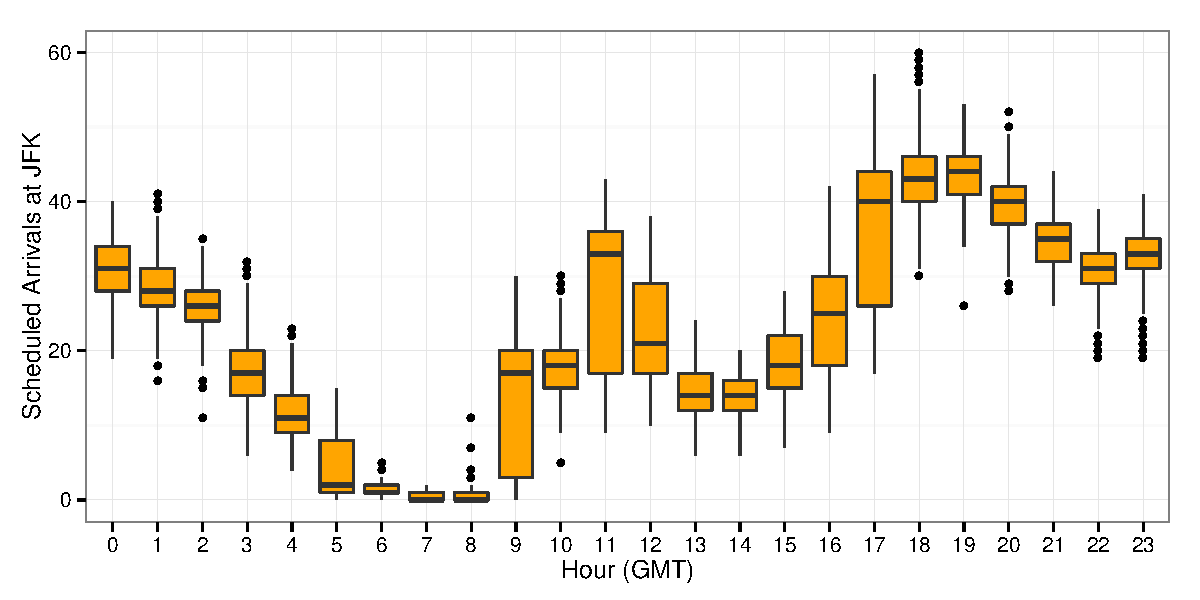
\includegraphics[scale=0.8125]{./figures/Fig1.pdf}
\caption{Counts of scheduled arrivals at JFK by hour.}
\label{default}
\end{center}
\end{figure}

\subsection{A PCA-Based Approach}
Another heuristic we explore for feature selection is based on Principal Component Analysis (PCA) and, similar to traffic biasing, converts hourly observations of a variable to a daily summary statistic.  PCA is used to select linear combinations of the 24 observed values of each variable per day which capture the largest possible variation between days (i.e. the first $n$ principal components).  Our earlier airspace-focused report describes, in more detail, how PCA can be used to automatically select features for a subsequent cluster analysis.  We summarize that discussion by noting that application of PCA is one way to reduce the dimensions of a dataset while maintaining as much of the differences between data points (here days) as possible.

Figure 2 shows the amount of variance explained by the first five principal components of a given day at JFK for various weather variables recorded in METAR data.  Note that all variables have strongly explanatory first principal component, but that the relevance of other principal components is variable. Figures similar to Figure 2 are worth exploring if an analyst wishes to utilize PCA-based feature selection. This methodology for feature selection is appropriate when expert judgement is missing or when the outputs of a clustering algorithm will be evaluated by comparing all available observations from a large data set.

\newpage\noindent
\begin{figure}[h]
\begin{center}
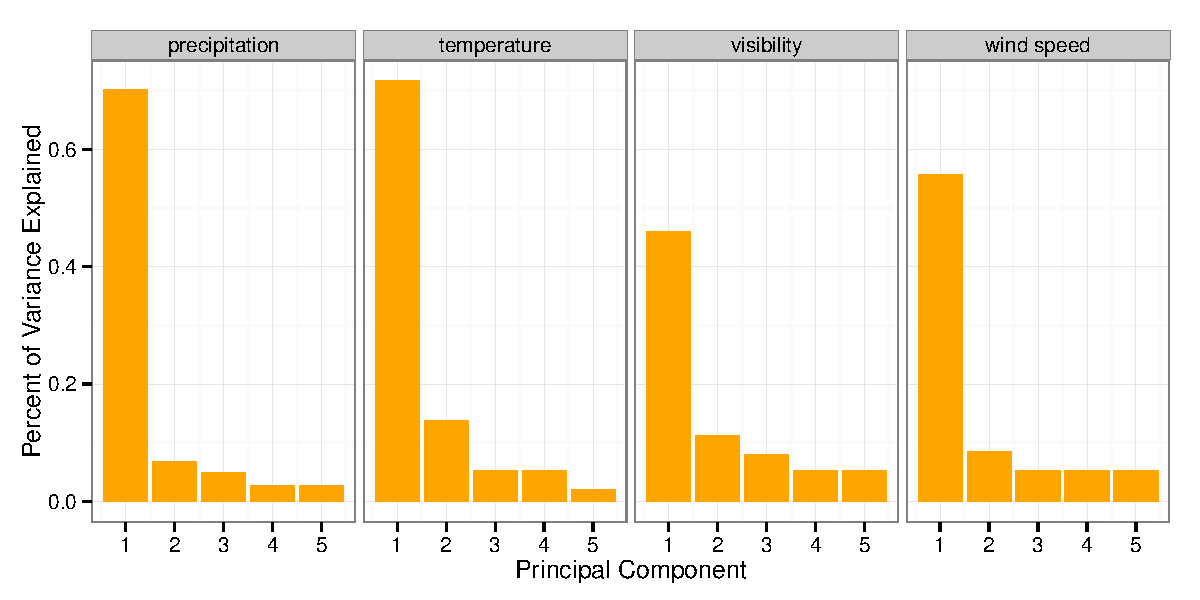
\includegraphics[scale=0.8125]{./figures/Fig2.pdf}
\caption{Variance explained by principal components for weather variables at JFK.}
\label{default}
\end{center}
\end{figure}

\section{Clustering Algorithms}
We described k-means and DBSCAN clustering approaches in our earlier airspace-focused report.  Neither algorithm is perfectly suited to our task here.  We instead apply a Partitioning Around Medoids (PAM) approach, as defined in \cite{silhouette}.  Parameters of this model include a number of clusters to find ($k$) and a way to measure distance between days based on feature data.  The distance measure need not be the Euclidean distance measure.  This is particularly important given that, among other variables, we are interested in wind direction data.  If the distance metric is properly specified, missing data are allowed.  If an analyst is unsure how to set $k$, he or she can try different values of $k$ and compare results.

The first step of our application of a PAM algorithm is to randomly select $k$ days during our study period.  These are the (initial) cluster centers.  For all other days, determine the cluster centers that they are closest to and assign the days to the respective clusters.  The ``quality'' of this clustering assignment is defined as the average distance from each day to its cluster center.

Next, consider each pair of points where exactly one of the points is currently a cluster center.  Imagine if the point that is not currently a cluster center becomes a cluster center while the other point in the pair loses its status as a cluster center.  This is called a ``swap.''  The single swap that does the most to improve the quality of the clustering assignment is performed.  The process repeats until no single swap will improve the quality of the final assignment.
\newpage\noindent
\section{Results and Discussion}
\subsection{Exploratory Analysis of Raw Data}
We here describe interesting results we obtain exploring raw weather and air traffic data provided by the data sources identified in Table 2.  Figure 1, shown earlier, highlights the different levels of scheduled arrivals by hour at JFK airport.  Similar results were obtained when looking at scheduled departures, observed operations, and at other airports in the New York area.  There was weaker evidence of such temporal patterns when looking at weather variables.  Figure 3, for example, shows parallel boxplots of observations of different weather variables (METAR data) at JFK arranged by hour.  Visibility looks to be slightly more of a problem in the morning hours (3am - 10am) while temperature and maybe windspeed are higher in the afternoon hours.
\begin{figure}[h]
\begin{center}
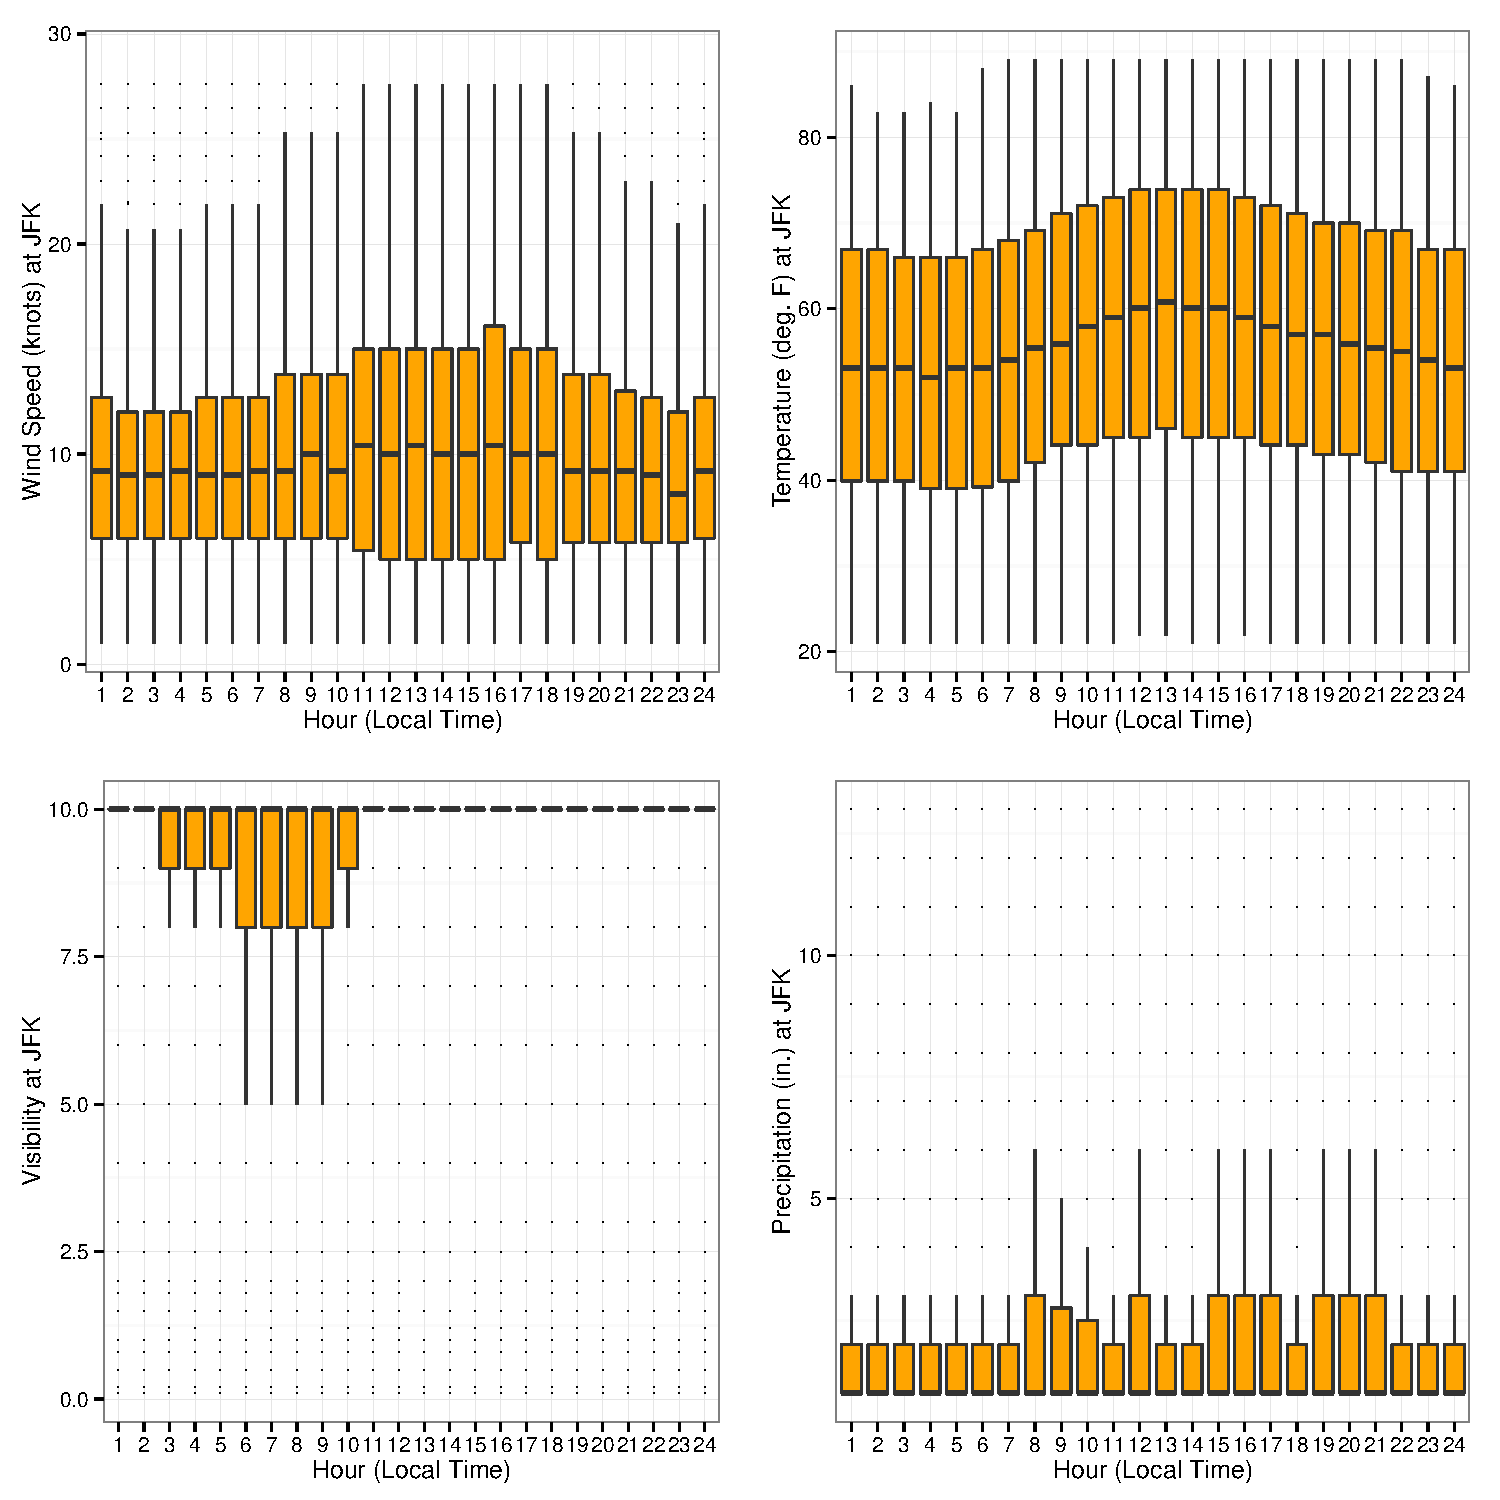
\includegraphics[scale=0.60]{./figures/Fig3.pdf}
\caption{Observations of different weather variables at JFK by hour.}
\label{default}
\end{center}
\end{figure}
\newpage\noindent
Results published in our airspace-focused report revealed strong seasonal patterns in weather data.  Figure 4 shows weak seasonality in airport specific data.  The same METAR data and weather variables used to create Figure 3 are shown here.  Wind speed looks to be highest from January to April and weakest from May to September.  Temperature, not surprisingly, exhibits strong seasonality.
\begin{figure}[h]
\begin{center}
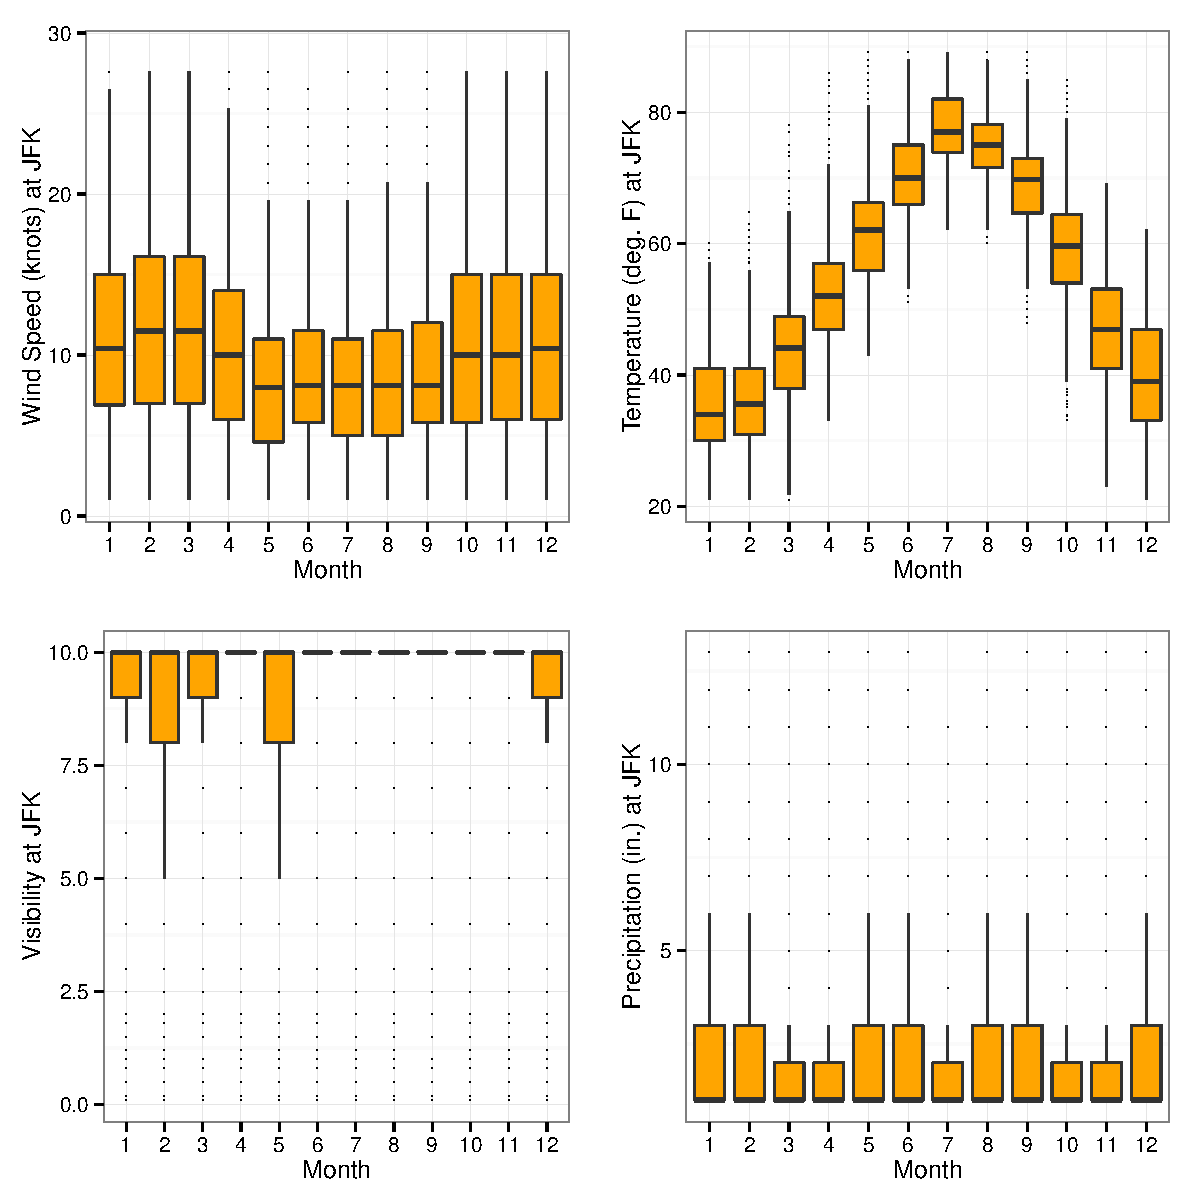
\includegraphics[scale=0.80]{./figures/Fig4.pdf}
\caption{Observations of different weather variables at JFK by month.}
\label{default}
\end{center}
\end{figure}
\par\noindent
There was minimal evidence of correlations within the set of weather and air traffic variables we collected, aside from trivial correlations between, for example, counts of arrivals and departures at an airport or observations of precipitation at JFK and LGA airports.
\newpage\noindent
\subsection{Analysis of Features and Results of Clustering}
We applied the knowledge-based feature selection methodology described previously to raw LAMP and ASPM data to yield features that describe the days in our study period, January 1, 2010 through December 31, 2013.  We use a total of 48 features, 12 describing scheduled air traffic and 36 describing forecast weather conditions, including:
\begin{itemize}
\item{scheduled arrivals at each relevant airport (JFK, EWR, \& LGA) during each of several key time windows (10:00-13:00 GMT, 13:00-16:00 GMT, 16:00-19:00 GMT, 19:00-22:00 GMT),}
\item{forecast visibility at each airport at selected times (00:00, 06:00, 12:00, 18:00 local time),}
\item{forecast wind speed at each airport at selected times, and}
\item{forecast wind direction at each airport at selected times.}
\end{itemize}
There were gaps in the LAMP data that made it impossible to define all of the features detailed above for every day in our study period.  A strength of the PAM algorithm for clustering is that it is able to cluster data containing missing values.  We applied the PAM clustering algorithm to our feature data various times.  We consistently scaled the data and used the Manhattan or $L_1$ distance metric.  We decided to do this after finding no reason to explicitly or implicitly weight certain features more than others.  We varied the number of clusters that the algorithm defined.  There are valid reasons for wanting to identify a greater number of more tightly defined clusters or a smaller number of clusters whose data points are less similar.  Using PAM ensured that identified clusters were centered around actual days within our study period.  Table 3 describes the days at the centers of our clusters when splitting our study period up into 10 clusters of similar days.  Dash marks indicate that there was no data available at the relevant time for the relevant variable.
\begin{table}[h]
\caption{Representative dates at airports in the New York area.}
\begin{center}
\begin{tabular}{|l|l|l|l|l|l|l|}
\hline
{\bf Date} & {\bf JFK} & {\bf EWR} & {\bf LGA} & {\bf JFK mean} & {\bf EWR} & {\bf LGA} \\
& {\bf scheduled} & {\bf arrivals} & {\bf arrivals} & {\bf forecast} & {\bf wind} & {\bf wind}\\
& {\bf arrivals} & & &  {\bf wind speed} & & \\
& {\bf (10:00-22:00 GMT)} & & & {\bf (knots)} & & \\
\hline
02 / 12 / 2010 & 326 & 331 & 345 & 0.0 & 0.0 & 0.0\\
\hline
06 / 22 / 2010 & 348 & 366 & 392 & 2.8 & 2.8 & 2.8\\
\hline
10 / 09 / 2010 & 339 & 308 & 222 & 2.2 & 2.2 & 2.2\\
\hline
05 / 10 / 2011 & 350 & 345 & 399 & - & - & -\\
\hline
06 / 05 / 2011 & 371 & 320 & 304 & - & - & -\\
\hline
09 / 14 / 2011 & 343 & 331 & 395 & 3.0 & 3.0 & 3.0\\
\hline
02 / 10 / 2012 & 317 & 323 & 356 & 0.5 & 0.5 & 0.5\\
\hline
05 / 15 / 2012 & 331 & 370 & 381 & 61.0 & 67.5 & 64.5\\
\hline
08 / 28 / 2012 & 358 & 362 & 388 & - & - & -\\
\hline
07 / 02 / 2013 & 362 & 352 & 344 & 42.5 & 44.0 & 44.0\\
\hline
\end{tabular}
\end{center}
\label{default}
\end{table}

Note that the identified `representative days' are relatively evenly distributed across the years and months of the study period.  There were high, low, and close to no winds forecast in the New York area during two, three, and two of the identified days, respectively.  It is important to point out that the data shown in Table 3 is derived from, but not the exact, data that was used to cluster the days.

In our airspace-focused report, we highlighted the fact that there was relatively weak `structure' in data sets describing days using features derived from scheduled air traffic and forecast weather data.  The same issue is relevant here.  Average silhouette width is the most commonly used measure of structure as it relates to cluster analysis and is described in \cite{silhouette}.  For each day $x$, let $a(x)$ be the average distance from $x$ to other days assigned to the same cluster in a given analysis.  Let $b(x)$ be the minimum, across the set of clusters that $x$ is not assigned to, of the average distance from $x$ to the days in the cluster.  The silhouette width of day $x$ is then defined as follows.\\

$$s(x) = \frac{b(x)-a(x)}{\max (a(x),b(x))}$$\\

The average silhouette width is the average of these values, across all days.  This metric reflects how well the days are described by the clusters to which they have been assigned.

Figure 5 shows the silhouette width obtained when applying PAM clustering to our feature data for various values of the parameter $k$ that sets the number of clusters to define.  It is generally accepted that a silhouette width of less than 0.25 indicates a lack of structure in data.  There is a remarkable lack of structure in our feature data.

\begin{figure}[h]
\begin{center}
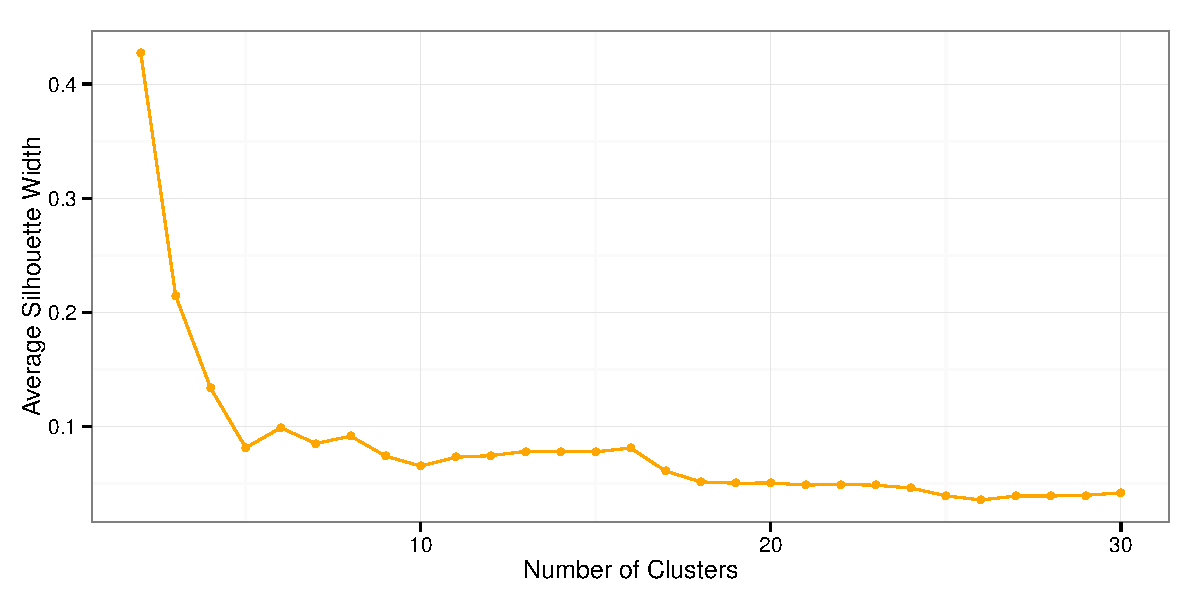
\includegraphics[scale=0.8125]{./figures/Fig5.pdf}
\caption{Average silhouette width as a function of k, looking at conditions at airports in the New York area.}
\label{default}
\end{center}
\end{figure}

The lack of structure in our data indicates that different days are not arranged into a set number of well defined clusters containing similar types of days, when looking at airport weather and traffic conditions in the New York area.  It would make intuitive sense if part of the problem stemmed from studying three different airports at once.  The data, however, show that there is a consistent lack of structure when looking at data that describe a single airport.  Figure 6 is similar to figure 5 but is based on apply a PAM clustering algorithm to data from JFK airport alone.

\begin{figure}[h]
\begin{center}
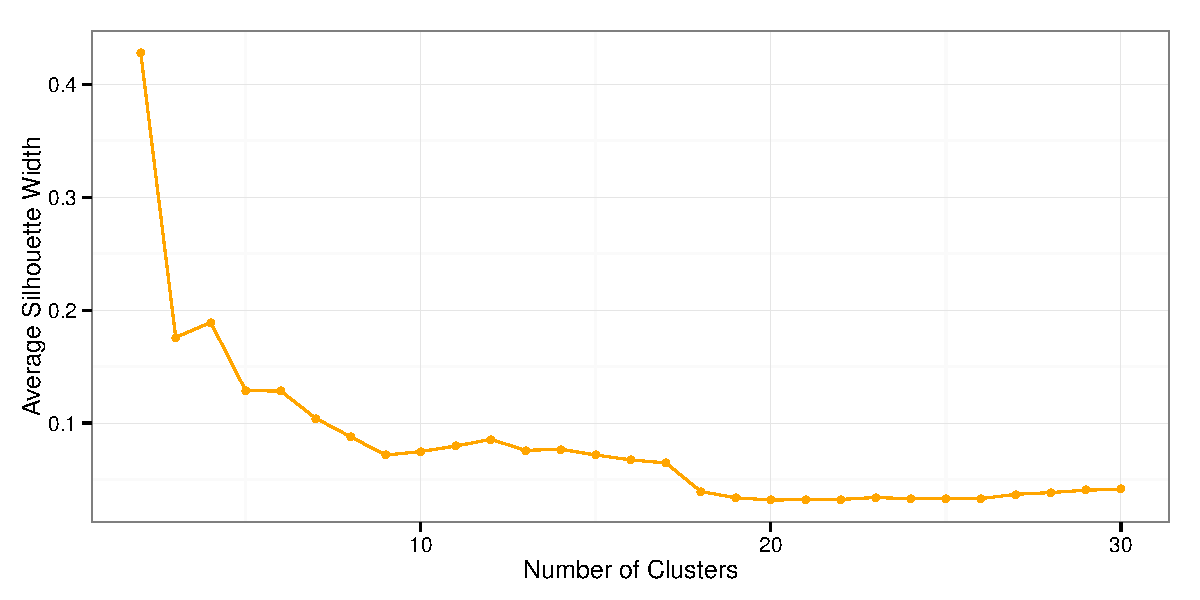
\includegraphics[scale=0.8125]{./figures/Fig6.pdf}
\caption{Average silhouette width as a function of k, looking at conditions at JFK airport alone.}
\label{default}
\end{center}
\end{figure}

%
% I commented out the pseudo-label and concurrency table writeup and tables.  I couldn't find an interesting and convincing story to tell here.
% -Ken
%
%When ground-truth labels are available, classification models can be assessed by various quantitative metrics that characterize the intra-cluster similarity of those labels versus the inter-cluster similarity of labels.  One example of such a metric is the RAND index, but there are various others.  More generally a ``confusion matrix" is a standard representation in Machine Learning to present the accuracy of an algorithm that models a categorial variable.  Typically, a model that has been fit using a training data set is asked to forecast the categorical variable in a distinct test data set.  The rows of the confusion matrix represent the actual values of the categorical variable in the test data set while the columns represent the model output values of the categorical variable using the model inputs from the test data set.  Each cell in the matrix is a count showing how many times the model predicted label x (column) when the actual observation was was label y (row).
%
%We propose a novel method to use categorical data as ``psuedo-labels" for each observation.  The data we use for these psuedo-labels are the observed ``Condition" data column of METAR data, a categorical value.  Each day (sample of our data-matrix) has 24 such values and we propose three types of concurrency tables which allow use to analyze the similarity within and between the clusters using the frequency of occurrence of those categorical values.
%
%The Condition data within METAR data describe weather conditions at an airport using a categorical variable.  The data are not ground-truth labels in the sense that we would explicitly seek to build a model of this data or claim that the data adequately summarize airport weather data for air traffic flow management initiative planning.  However, it is worthwhile to compare the results of cluster analysis to the Condition data, to see if, for example, days with the Condition label of ``Thunderstorm'' appear in one cluster while days with the Condition label of ``Clear'' appear in another cluster.  To explore the relationship between the METAR Condition data and identified clusters, we created concurrency tables.  The idea is similar to that of the Confusion Matrix described above.  Each row in a concurrency table refers to a specific Condition label and each column to a specific cluster output by a clustering algorithm.  Each cell in a concurrency table contains a count of the number of times a day was assigned to a specific Condition label (row) according to observed METAR data and a specific cluster (column) according to the results of a specific form of cluster analysis.
%
%Using results from:
%/Users/ashah/NoBackup/code/nasa/results/JFKexpert_kmeans_5.csv
%Day-Aggregrated counts:
%\begin{tabular}{lrrrrr}
%\toprule
%{} &     1 &     2 &     3 &      4 &      5 \\
%\midrule
%Blowing Snow                  &   - &   - &   - &      2 &      2 \\
%Clear                         &   490 &   548 &  1936 &   2651 &   2674 \\
%Fog                           &     5 &   230 &   233 &    238 &    462 \\
%Haze                          &    55 &   181 &   202 &    207 &    310 \\
%Heavy Rain                    &    22 &    74 &    80 &    155 &    238 \\
%Heavy Snow                    &   - &     4 &     4 &      6 &     24 \\
%Heavy Thunderstorms and Rain  &    36 &    62 &    66 &     71 &     86 \\
%Ice Pellets                   &   - &     3 &     3 &      5 &      6 \\
%Light Drizzle                 &     9 &   144 &   170 &    191 &    458 \\
%Light Freezing Drizzle        &   - &     7 &     7 &      7 &     45 \\
%Light Freezing Rain           &   - &     4 &     4 &      4 &     36 \\
%Light Ice Pellets             &   - &     3 &     4 &      4 &     24 \\
%Light Rain                    &   347 &   874 &  1330 &   1867 &   2799 \\
%Light Rain Showers            &   - &   - &   - &      1 &      1 \\
%Light Snow                    &   - &   194 &   304 &    463 &    814 \\
%Light Thunderstorms and Rain  &    70 &   100 &   123 &    128 &    146 \\
%Light Thunderstorms and Snow  &   - &   - &   - &    - &      1 \\
%Mist                          &   - &    12 &    12 &     12 &     27 \\
%Mostly Cloudy                 &  3410 &  4483 &  8639 &  11069 &  11501 \\
%Overcast                      &  1135 &  2319 &  4619 &   5825 &   7271 \\
%Partly Cloudy                 &   950 &  1075 &  2924 &   4404 &   4455 \\
%Patches of Fog                &   - &     4 &     4 &      4 &      5 \\
%Rain                          &    40 &   150 &   184 &    264 &    481 \\
%Scattered Clouds              &  2068 &  2448 &  4859 &   6562 &   6659 \\
%Shallow Fog                   &     2 &     2 &     2 &      2 &      2 \\
%Smoke                         &   - &   - &     1 &      1 &      1 \\
%Snow                          &   - &    15 &    18 &     40 &     71 \\
%Squalls                       &   - &   - &     1 &      1 &      1 \\
%Thunderstorm                  &    47 &    51 &    62 &     67 &     68 \\
%Thunderstorms and Rain        &    24 &    35 &    40 &     47 &     53 \\
%Thunderstorms with Small Hail &   - &     1 &     1 &      1 &      1 \\
%Unknown                       &     5 &     7 &    11 &     16 &     20 \\
%\bottomrule
%\end{tabular}
%
%
%Day-Most frequent counts:
%\begin{tabular}{lrrrrr}
%\toprule
%{} &     1 &     2 &     3 &     4 &     5 \\
%\midrule
%Clear                  &   117 &   117 &   655 &   899 &   899 \\
%Fog                    &   - &    72 &    72 &    72 &   132 \\
%Haze                   &   - &    10 &    10 &    10 &    33 \\
%Heavy Rain             &   - &   - &   - &    25 &    25 \\
%Light Drizzle          &   - &    20 &    20 &    20 &    54 \\
%Light Freezing Drizzle &   - &   - &   - &   - &    23 \\
%Light Rain             &    48 &   282 &   397 &   566 &  1112 \\
%Light Snow             &   - &   147 &   196 &   262 &   551 \\
%Mostly Cloudy          &  2616 &  3205 &  6215 &  7825 &  7903 \\
%Overcast               &   453 &  1181 &  2337 &  2885 &  3837 \\
%Partly Cloudy          &   334 &   358 &  1146 &  1837 &  1837 \\
%Rain                   &   - &     9 &     9 &     9 &     9 \\
%Scattered Clouds       &  1113 &  1186 &  2126 &  2828 &  2852 \\
%Snow                   &   - &   - &   - &    12 &    22 \\
%\bottomrule
%\end{tabular}
%
%
%Day-Least frequent counts:
%\begin{tabular}{lrrrrr}
%\toprule
%{} &    1 &    2 &    3 &    4 &    5 \\
%\midrule
%Clear                        &   73 &   79 &  252 &  343 &  348 \\
%Fog                          &  - &   12 &   12 &   13 &   17 \\
%Haze                         &   11 &   22 &   35 &   38 &   48 \\
%Heavy Rain                   &    4 &   22 &   25 &   35 &   60 \\
%Heavy Snow                   &  - &    4 &    4 &    4 &    4 \\
%Heavy Thunderstorms and Rain &    5 &    7 &    7 &    9 &   14 \\
%Ice Pellets                  &  - &  - &  - &  - &    1 \\
%Light Drizzle                &    1 &   14 &   23 &   30 &   66 \\
%Light Freezing Drizzle       &  - &  - &  - &  - &    2 \\
%Light Freezing Rain          &  - &  - &  - &  - &    1 \\
%Light Ice Pellets            &  - &    1 &    2 &    2 &    7 \\
%Light Rain                   &   50 &   76 &  150 &  205 &  220 \\
%Light Rain Showers           &  - &  - &  - &    1 &    1 \\
%Light Snow                   &  - &    3 &    6 &   26 &   27 \\
%Light Thunderstorms and Rain &   18 &   22 &   28 &   30 &   30 \\
%Light Thunderstorms and Snow &  - &  - &  - &  - &    1 \\
%Mist                         &  - &   10 &   10 &   10 &   14 \\
%Mostly Cloudy                &  141 &  158 &  366 &  508 &  534 \\
%Overcast                     &   94 &  109 &  281 &  383 &  397 \\
%Partly Cloudy                &  189 &  206 &  486 &  661 &  665 \\
%Patches of Fog               &  - &  - &  - &  - &    1 \\
%Rain                         &   15 &   29 &   40 &   60 &   90 \\
%Scattered Clouds             &  178 &  198 &  603 &  752 &  769 \\
%Shallow Fog                  &    2 &    2 &    2 &    2 &    2 \\
%Smoke                        &  - &  - &    1 &    1 &    1 \\
%Snow                         &  - &  - &  - &  - &    3 \\
%Squalls                      &  - &  - &    1 &    1 &    1 \\
%Thunderstorm                 &    3 &    5 &    5 &    5 &    5 \\
%Thunderstorms and Rain       &   10 &   18 &   19 &   22 &   27 \\
%Unknown                      &    1 &    2 &    4 &    4 &    6 \\
%\bottomrule
%\end{tabular}
%
%
%Condition Concurrency Tables for airport:EWR
%
%Using results from:
%/Users/ashah/NoBackup/code/nasa/results/EWRexpert_kmeans_5.csv
%
%Day-Aggregrated counts:
%\begin{tabular}{lrrrrr}
%\toprule
%{} &     1 &     2 &     3 &     4 &      5 \\
%\midrule
%Blowing Snow                        &   - &   - &    10 &    10 &     10 \\
%Clear                               &   516 &  1446 &  1514 &  1546 &   3176 \\
%Fog                                 &   - &   - &    70 &   147 &    149 \\
%Haze                                &    29 &    35 &   191 &   416 &    525 \\
%Heavy Ice Pellets                   &   - &   - &   - &     1 &      1 \\
%Heavy Rain                          &     5 &    20 &    90 &   242 &    284 \\
%Heavy Snow                          &   - &     1 &    18 &    53 &     53 \\
%Heavy Thunderstorms and Rain        &     3 &    15 &    31 &    56 &    128 \\
%Ice Pellets                         &   - &   - &     3 &    12 &     12 \\
%Light Drizzle                       &     4 &    25 &   158 &   618 &    656 \\
%Light Freezing Drizzle              &   - &   - &     7 &    48 &     48 \\
%Light Freezing Rain                 &   - &   - &    17 &    52 &     52 \\
%Light Ice Pellets                   &     3 &     8 &    14 &    39 &     41 \\
%Light Rain                          &   151 &   547 &  1217 &  2633 &   3438 \\
%Light Rain Showers                  &   - &   - &   - &     1 &      1 \\
%Light Snow                          &    45 &   143 &   434 &   834 &    881 \\
%Light Thunderstorms and Ice Pellets &   - &   - &   - &     2 &      2 \\
%Light Thunderstorms and Rain        &     3 &    32 &    54 &    88 &    199 \\
%Mist                                &   - &   - &   - &     3 &      3 \\
%Mostly Cloudy                       &  1634 &  4074 &  5015 &  5404 &  11420 \\
%Overcast                            &   886 &  2021 &  3168 &  4695 &   7838 \\
%Partly Cloudy                       &   551 &  1833 &  1947 &  1988 &   3679 \\
%Rain                                &     4 &    60 &   182 &   492 &    560 \\
%Scattered Clouds                    &   881 &  2537 &  2835 &  2932 &   5746 \\
%Smoke                               &   - &   - &   - &   - &      1 \\
%Snow                                &     6 &    11 &    41 &    91 &     91 \\
%Thunderstorm                        &     5 &    27 &    44 &    47 &    121 \\
%Thunderstorms and Rain              &     4 &    17 &    30 &    55 &     94 \\
%Unknown                             &     4 &    12 &    14 &    15 &     17 \\
%\bottomrule
%\end{tabular}
%Day-Most frequent counts:
%\begin{tabular}{lrrrrr}
%\toprule
%{} &     1 &     2 &     3 &     4 &     5 \\
%\midrule
%Blowing Snow           &   - &   - &     9 &     9 &     9 \\
%Clear                  &   225 &   613 &   613 &   613 &  1235 \\
%Fog                    &   - &   - &    10 &    32 &    32 \\
%Haze                   &     8 &     8 &    40 &   118 &   137 \\
%Heavy Rain             &   - &   - &    15 &    15 &    15 \\
%Heavy Snow             &   - &   - &   - &    17 &    17 \\
%Light Drizzle          &   - &   - &    11 &   152 &   152 \\
%Light Freezing Drizzle &   - &   - &   - &    25 &    25 \\
%Light Freezing Rain    &   - &   - &    10 &    10 &    10 \\
%Light Rain             &    17 &   146 &   485 &  1457 &  1594 \\
%Light Snow             &    14 &    51 &   295 &   627 &   639 \\
%Mostly Cloudy          &  1113 &  2869 &  3367 &  3437 &  7909 \\
%Overcast               &   510 &   953 &  1627 &  2476 &  4220 \\
%Partly Cloudy          &   199 &   670 &   670 &   670 &  1222 \\
%Rain                   &   - &   - &   - &    44 &    44 \\
%Scattered Clouds       &   362 &  1017 &  1083 &  1083 &  2154 \\
%\bottomrule
%\end{tabular}
%Day-Least frequent counts:
%\begin{tabular}{lrrrrr}
%\toprule
%{} &    1 &    2 &    3 &    4 &    5 \\
%\midrule
%Blowing Snow                 &  - &  - &    1 &    1 &    1 \\
%Clear                        &   55 &  144 &  145 &  153 &  371 \\
%Fog                          &  - &  - &    8 &   12 &   12 \\
%Haze                         &    5 &    8 &   31 &   41 &   58 \\
%Heavy Ice Pellets            &  - &  - &  - &    1 &    1 \\
%Heavy Rain                   &    1 &    8 &   15 &   56 &   63 \\
%Heavy Snow                   &  - &    1 &    2 &    3 &    3 \\
%Heavy Thunderstorms and Rain &  - &  - &    1 &    4 &    7 \\
%Light Drizzle                &    1 &    8 &   24 &   53 &   66 \\
%Light Freezing Drizzle       &  - &  - &    1 &    2 &    2 \\
%Light Ice Pellets            &  - &  - &    1 &    4 &    4 \\
%Light Rain                   &   14 &   56 &   75 &  105 &  191 \\
%Light Rain Showers           &  - &  - &  - &    1 &    1 \\
%Light Snow                   &   12 &   28 &   46 &   55 &   61 \\
%Light Thunderstorms and Rain &  - &    7 &   12 &   16 &   25 \\
%Mist                         &  - &  - &  - &    1 &    1 \\
%Mostly Cloudy                &   95 &  233 &  247 &  266 &  511 \\
%Overcast                     &   98 &  191 &  204 &  253 &  519 \\
%Partly Cloudy                &   96 &  272 &  290 &  299 &  614 \\
%Rain                         &    2 &   13 &   28 &   68 &   90 \\
%Scattered Clouds             &  126 &  246 &  283 &  302 &  686 \\
%Smoke                        &  - &  - &  - &  - &    1 \\
%Snow                         &  - &  - &    2 &    9 &    9 \\
%Thunderstorm                 &  - &    3 &    4 &    5 &   17 \\
%Thunderstorms and Rain       &    2 &    5 &   10 &   13 &   34 \\
%Unknown                      &  - &    7 &    8 &    8 &   10 \\
%\bottomrule
%\end{tabular}
%Condition Concurrency Tables for airport:LGA
%Using results from:/Users/ashah/NoBackup/code/nasa/results/LGAexpert_kmeans_5.csv
%
%Day-Aggregrated counts:
%\begin{tabular}{lrrrrr}
%\toprule
%{} &     1 &     2 &     3 &     4 &      5 \\
%\midrule
%Blowing Snow                  &   - &   - &   - &     1 &      1 \\
%Clear                         &   605 &  2618 &  2630 &  3566 &   3618 \\
%Drizzle                       &   - &   - &     1 &     1 &      1 \\
%Fog                           &     5 &     5 &    17 &    19 &    173 \\
%Haze                          &    40 &   133 &   183 &   193 &    327 \\
%Heavy Rain                    &    19 &    65 &   226 &   276 &    354 \\
%Heavy Snow                    &   - &   - &    21 &    21 &     26 \\
%Heavy Thunderstorms and Rain  &     2 &    52 &    84 &    86 &     91 \\
%Ice Pellets                   &   - &   - &   - &   - &      3 \\
%Light Drizzle                 &    19 &    58 &   225 &   255 &    374 \\
%Light Freezing Drizzle        &     3 &     3 &     8 &     8 &     25 \\
%Light Freezing Rain           &     1 &     1 &    25 &    25 &     66 \\
%Light Ice Pellets             &     3 &     9 &    19 &    20 &     21 \\
%Light Rain                    &   176 &   956 &  2143 &  2565 &   3161 \\
%Light Rain Showers            &   - &     1 &     1 &     1 &      1 \\
%Light Snow                    &   115 &   172 &   577 &   703 &    955 \\
%Light Thunderstorms and Rain  &     8 &    87 &   110 &   116 &    129 \\
%Light Thunderstorms and Snow  &   - &   - &     2 &     2 &      2 \\
%Mist                          &     3 &     3 &     3 &     3 &     26 \\
%Mostly Cloudy                 &  1823 &  7653 &  7940 &  9819 &  10413 \\
%Overcast                      &  1084 &  4695 &  5847 &  7214 &   8654 \\
%Partly Cloudy                 &   632 &  2851 &  2883 &  4185 &   4262 \\
%Rain                          &    14 &    91 &   418 &   483 &    622 \\
%Scattered Clouds              &   964 &  4073 &  4131 &  5424 &   5623 \\
%Snow                          &     6 &     6 &    54 &    71 &    106 \\
%Thunderstorm                  &     6 &    72 &    73 &    75 &     78 \\
%Thunderstorms and Ice Pellets &   - &   - &     1 &     1 &      1 \\
%Thunderstorms and Rain        &     8 &    32 &    49 &    56 &     57 \\
%Unknown                       &   - &     2 &     2 &     4 &      4 \\
%\bottomrule
%\end{tabular}
%
%Day-Most frequent counts:
%\begin{tabular}{lrrrrr}
%\toprule
%{} &     1 &     2 &     3 &     4 &     5 \\
%\midrule
%Clear               &   271 &  1253 &  1253 &  1653 &  1666 \\
%Haze                &   - &   - &   - &   - &    34 \\
%Light Drizzle       &   - &   - &    41 &    41 &    48 \\
%Light Freezing Rain &   - &   - &    13 &    13 &    44 \\
%Light Rain          &    27 &   190 &   947 &  1031 &  1297 \\
%Light Snow          &    54 &    65 &   412 &   470 &   671 \\
%Mostly Cloudy       &  1299 &  5344 &  5414 &  6465 &  6651 \\
%Overcast            &   605 &  2839 &  3512 &  4318 &  5367 \\
%Partly Cloudy       &   238 &  1010 &  1010 &  1655 &  1655 \\
%Rain                &   - &     9 &    48 &    48 &    63 \\
%Scattered Clouds    &   389 &  1395 &  1395 &  1885 &  1925 \\
%\bottomrule
%\end{tabular}
%
%Day-Least frequent counts:
%\begin{tabular}{lrrrrr}
%\toprule
%{} &    1 &    2 &    3 &    4 &    5 \\
%\midrule
%Blowing Snow                 &  - &  - &  - &    1 &    1 \\
%Clear                        &   68 &  354 &  356 &  459 &  466 \\
%Drizzle                      &  - &  - &    1 &    1 &    1 \\
%Fog                          &    1 &    1 &    5 &    5 &    6 \\
%Haze                         &    6 &   22 &   31 &   31 &   55 \\
%Heavy Rain                   &    1 &   11 &   29 &   38 &   45 \\
%Heavy Snow                   &  - &  - &    8 &    8 &    8 \\
%Heavy Thunderstorms and Rain &  - &    4 &    6 &    7 &    8 \\
%Light Drizzle                &    4 &   12 &   34 &   44 &   72 \\
%Light Freezing Drizzle       &  - &  - &    1 &    1 &    4 \\
%Light Freezing Rain          &    1 &    1 &    1 &    1 &    1 \\
%Light Ice Pellets            &    1 &    2 &    3 &    4 &    5 \\
%Light Rain                   &   19 &  152 &  187 &  244 &  254 \\
%Light Rain Showers           &  - &    1 &    1 &    1 &    1 \\
%Light Snow                   &   10 &   21 &   22 &   28 &   29 \\
%Light Thunderstorms and Rain &    3 &   21 &   22 &   22 &   27 \\
%Mist                         &    3 &    3 &    3 &    3 &   11 \\
%Mostly Cloudy                &  107 &  309 &  329 &  441 &  454 \\
%Overcast                     &   66 &  266 &  280 &  362 &  367 \\
%Partly Cloudy                &  115 &  453 &  461 &  571 &  579 \\
%Rain                         &    4 &   25 &   46 &   58 &   67 \\
%Scattered Clouds             &  133 &  557 &  567 &  687 &  718 \\
%Snow                         &  - &  - &    2 &    4 &    6 \\
%Thunderstorm                 &    3 &   12 &   12 &   12 &   12 \\
%Thunderstorms and Rain       &    4 &   12 &   21 &   21 &   21 \\
%\bottomrule
%\end{tabular}
\section{Conclusion}
We have identified sets of similar days where similarity is defined in terms of key features of Localized Aviation MOS (Model Output Statistics) Product and Aviation System Performance Metrics data describing forecast weather and scheduled air traffic at airport in the New York area.  Our results and methodology can be used to study similar days or define representative days.  We note, however, that there is a lack of structure in the feature data we use to define similar days.  In other words, the actual conditions observed at airports in the New York area are not naturally or cleanly arranged into clear clusters of similar types of days.

More generally, we have surveyed the past and potential future use of clustering and classifying analyses in air traffic flow management research.  We recommend the use of TAF, METAR, LAMP, ASPM, ASDI, and ATFMI advisory data in such analyses.  We recommend the use of classification / supervised-learning algorithms if the goal is to model or forecast current planning or operations.  We recommend the use of the PAM algorithm if the goal is to instead explore data describing conditions at airports.  We find the key step in clustering and classifying analyses is the feature selection step, when the raw data sources listed above are processed to yield descriptive statistics that can be used as inputs for established clustering and classifying algorithms  We present three methodologies for feature selection: a PCA-based methodology, a traffic-biasing methodology, and a knowledge-based methodology.  The third approach offers the most promise, and further research should be devoted to identifying features relevant for current air traffic flow management planning and operations.

In the future, we will explore TAF and ATFMI advisory data recently made available to us.  We will also begin clustering and classifying days based on conditions at airports and in the airspace around the New York area.  This will require building off this report and a similar prior report focusing on the airspace.  Once we can confidently identify similar days based on all the conditions relevant to air traffic flow management in the New York area, we will examine what initiatives were initiated within clusters of similar days and what the results of these initiatives were.  The final result will be an analysis of the costs and benefits of alternate air traffic flow management initiatives that takes into account the distinct conditions faced during initiative planning and operations on different days. 
\bibliographystyle{abbrv}
\bibliography{all}
\end{document} 